
\chapter{Appendix: Atlas of Levelable Graphs} \label{appendix}

\section*{Non-levelable graphs on 6 vertices}

\begin{figure}[h!]
    {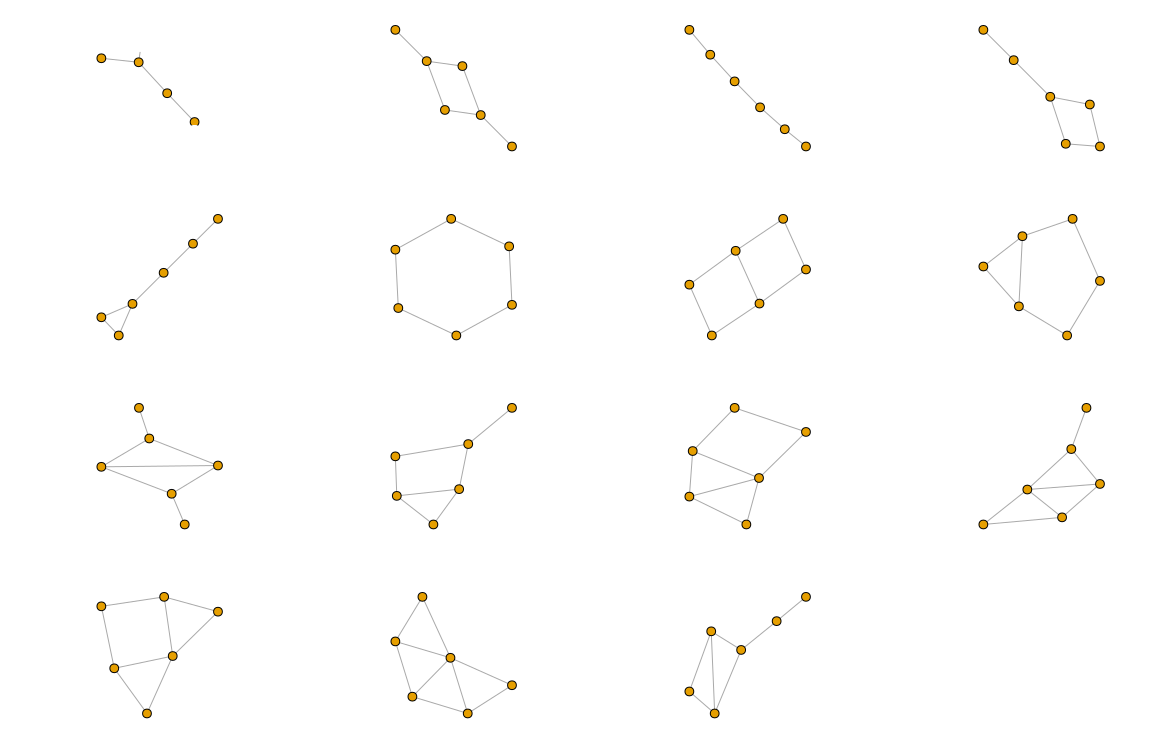
\includegraphics[width=1\linewidth]{atlas/atlas6.png}} 
\end{figure}

\section*{Non-levelable graphs on 7 vertices}
\vspace{-0.5cm}
\begin{figure}[h!]
    {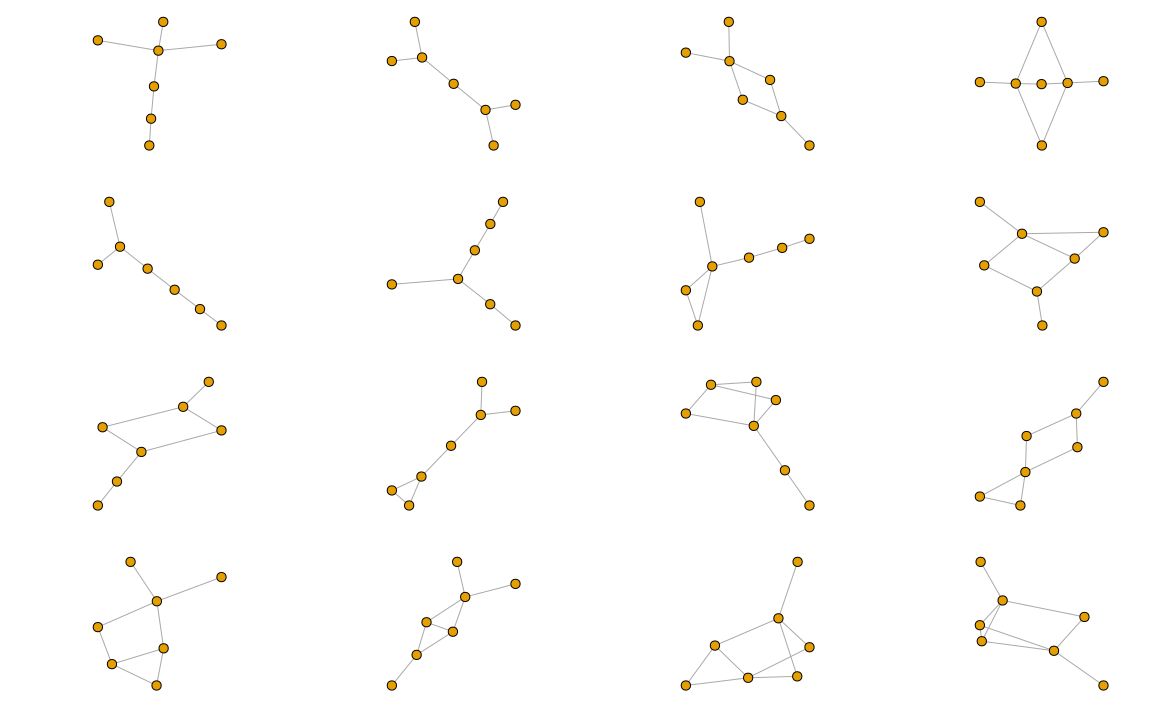
\includegraphics[width=0.95\linewidth]{atlas/atlas7-1.png}} 
\end{figure}

\begin{figure}[h!]
	\subfloat
    {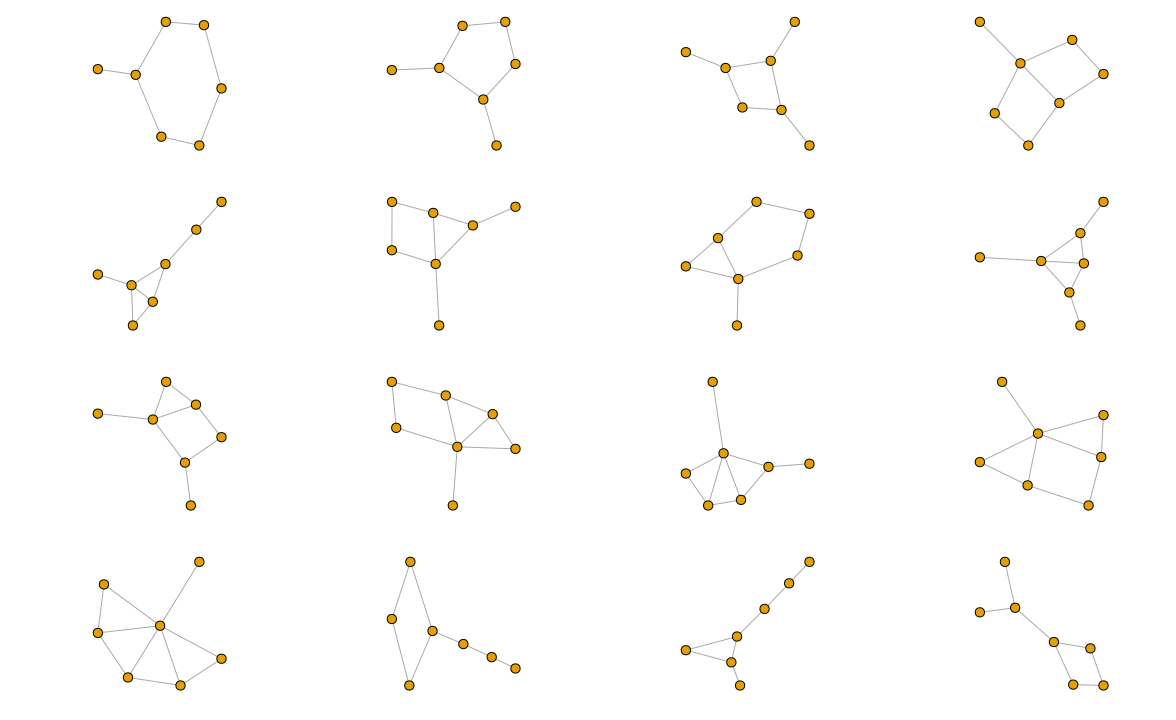
\includegraphics[width=0.95\linewidth]{atlas/atlas7-2.png}} \\
    \subfloat
    {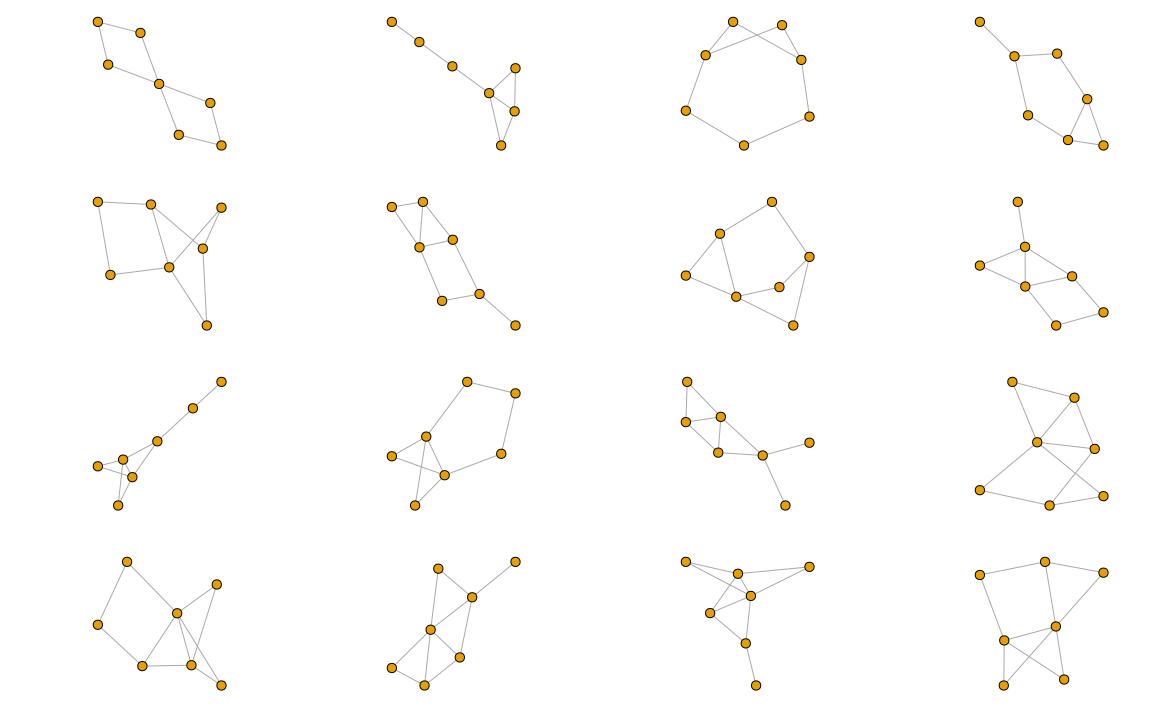
\includegraphics[width=0.95\linewidth]{atlas/atlas7-3.png}} \\
	\subfloat
    {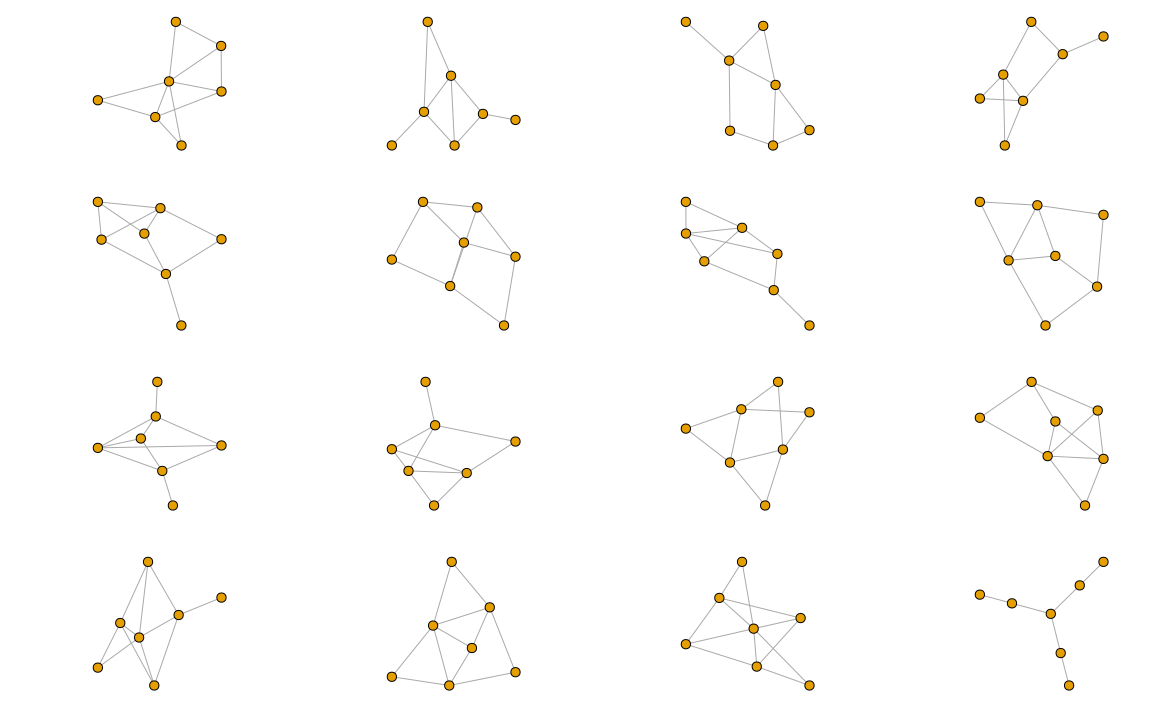
\includegraphics[width=0.95\linewidth]{atlas/atlas7-4.png}} 
\end{figure}

\begin{figure}[h!]
    \subfloat
    {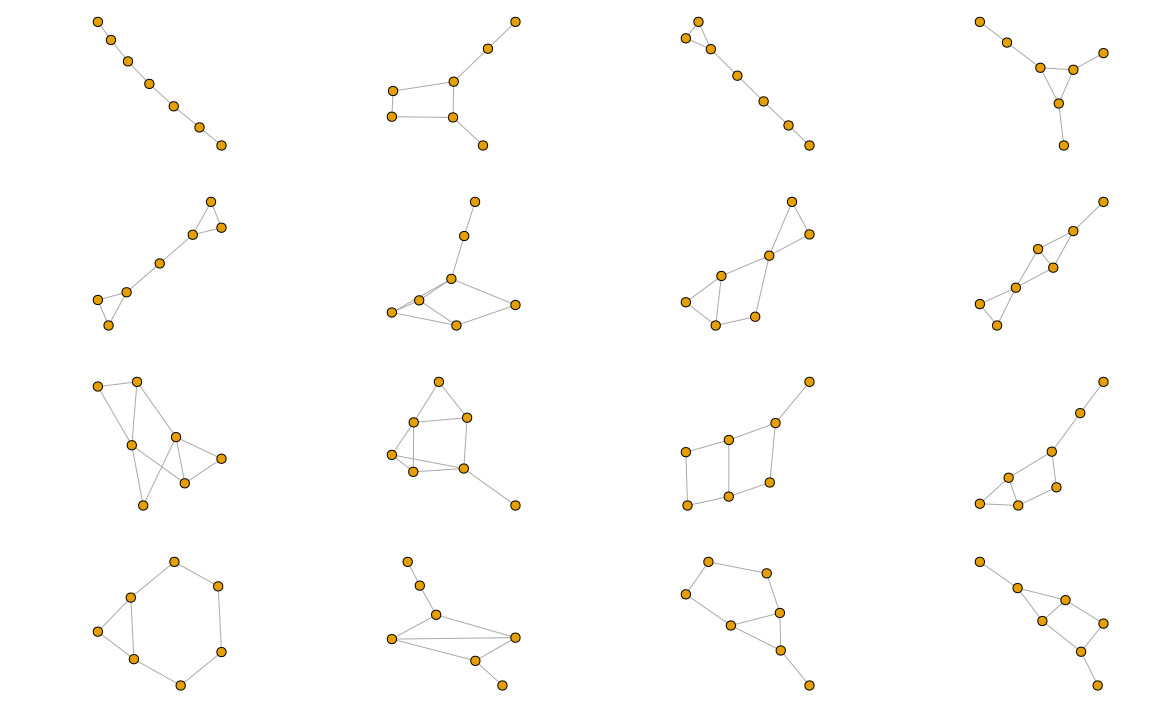
\includegraphics[width=0.95\linewidth]{atlas/atlas7-5.png}} \\
	\subfloat
    {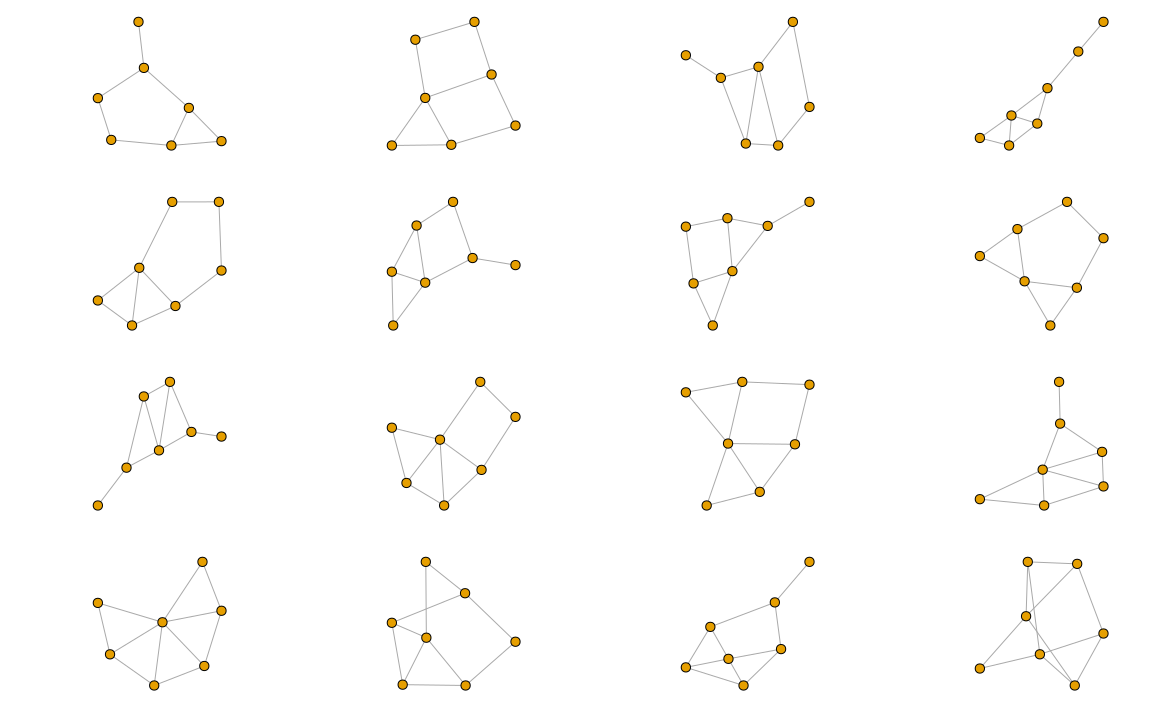
\includegraphics[width=0.95\linewidth]{atlas/atlas7-6.png}} \\
	\subfloat
    {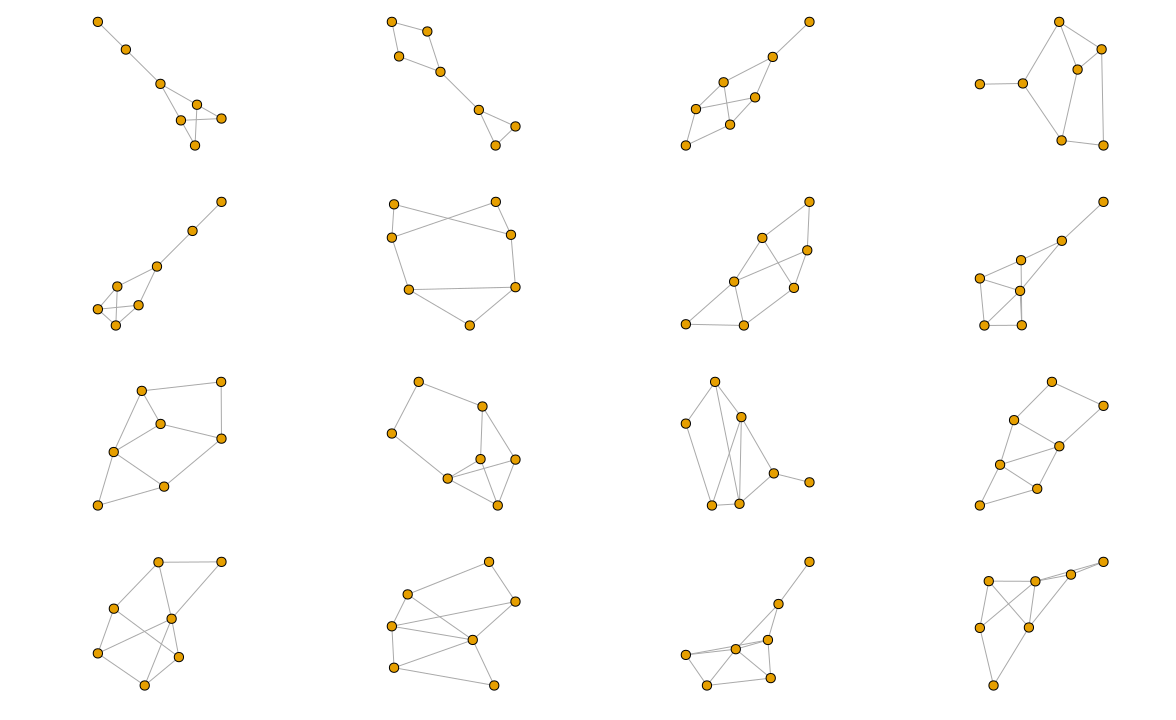
\includegraphics[width=0.95\linewidth]{atlas/atlas7-7.png}} 
\end{figure}

\begin{figure}[h!]
	\subfloat
	{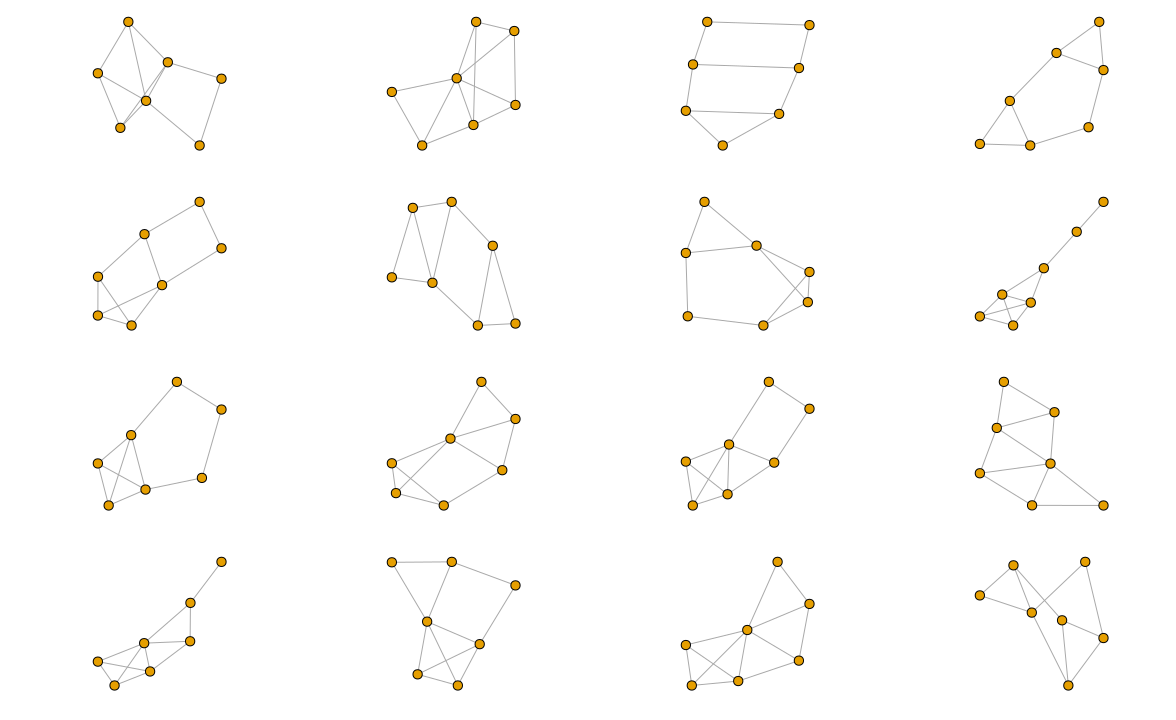
\includegraphics[width=0.95\linewidth]{atlas/atlas7-8.png}} \\
	\subfloat
    {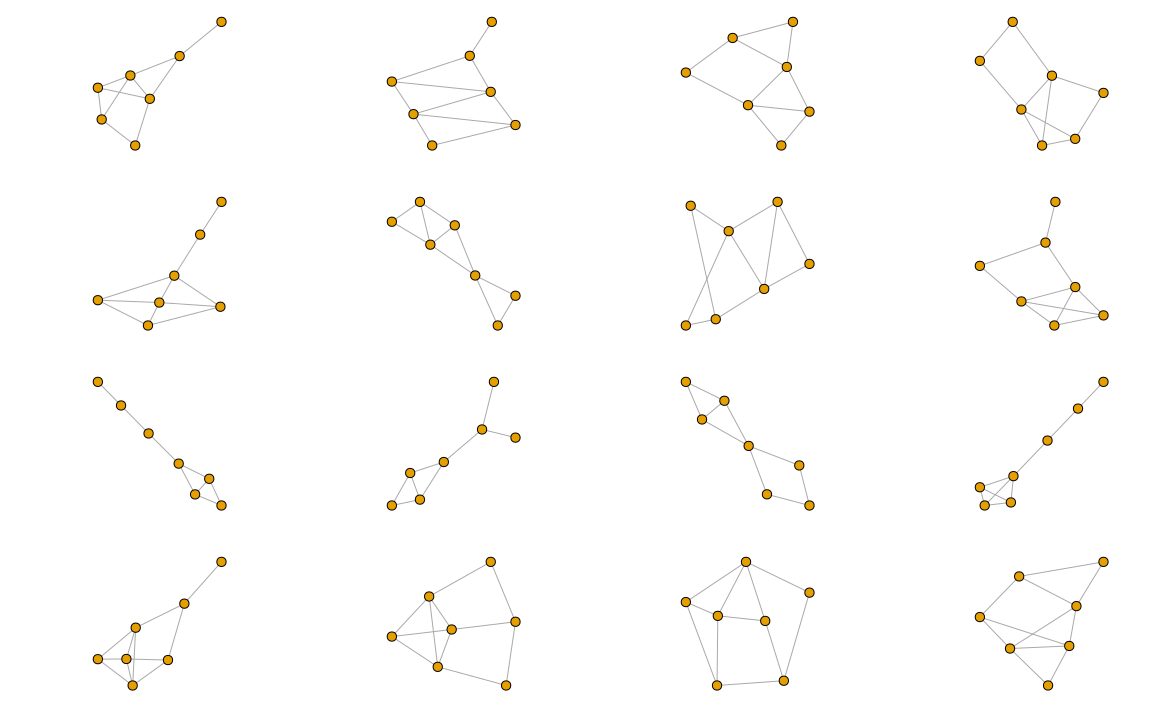
\includegraphics[width=0.95\linewidth]{atlas/atlas7-9.png}} \\
    \subfloat
    {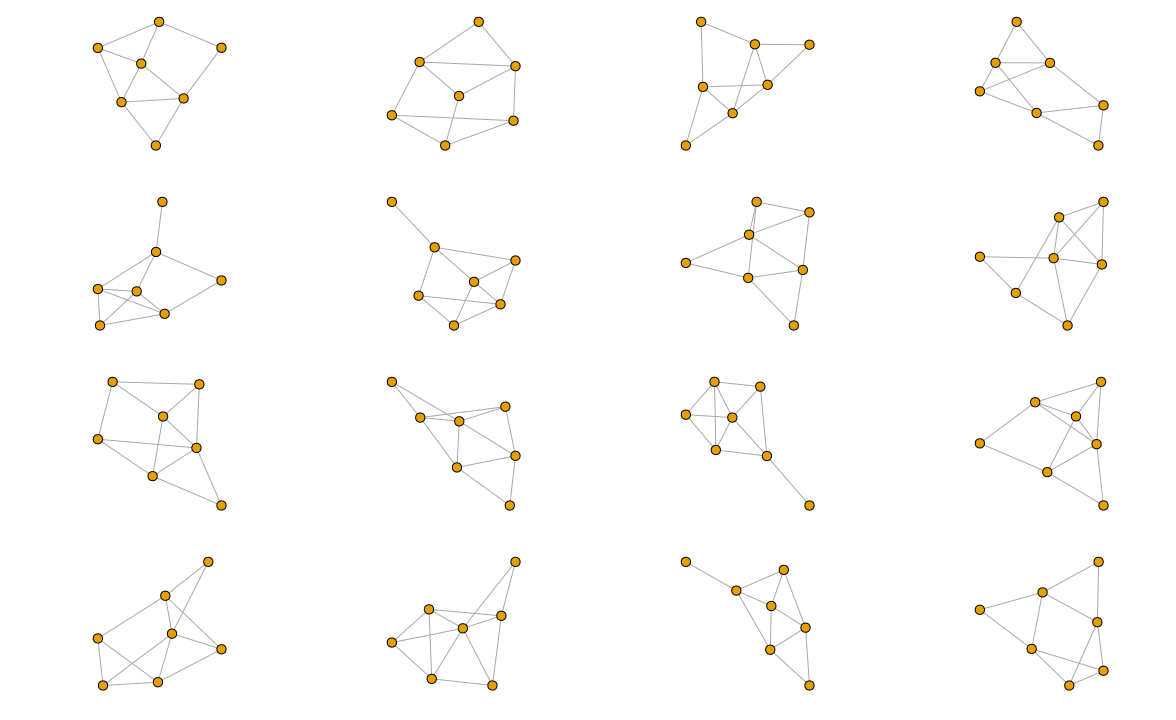
\includegraphics[width=0.95\linewidth]{atlas/atlas7-10.png}}
\end{figure}

\begin{figure}[h!]
	\subfloat
	{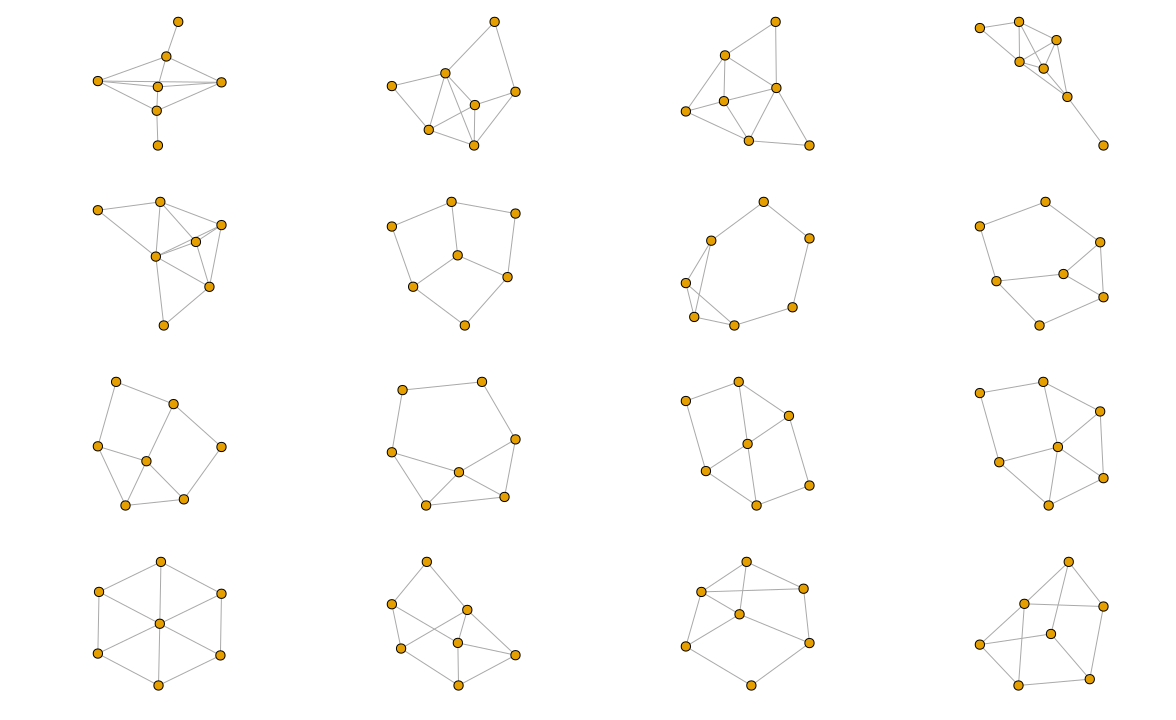
\includegraphics[width=0.95\linewidth]{atlas/atlas7-11.png}} \\
	\subfloat
    {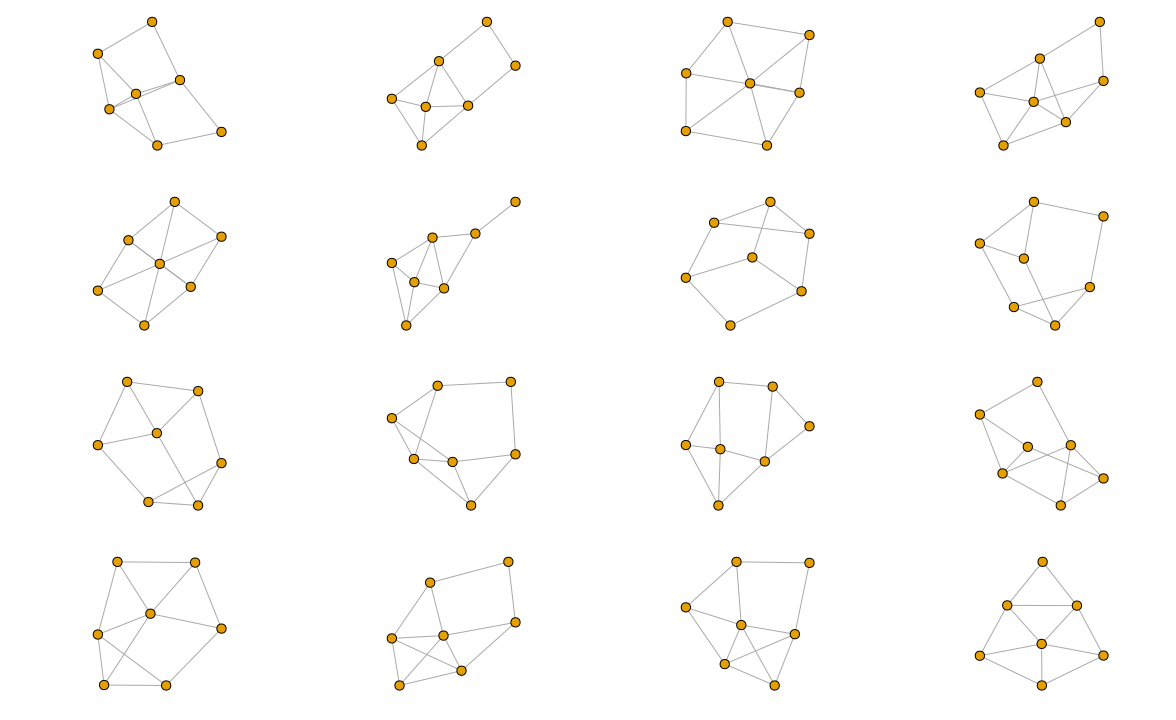
\includegraphics[width=0.95\linewidth]{atlas/atlas7-12.png}} \\
    \subfloat
    {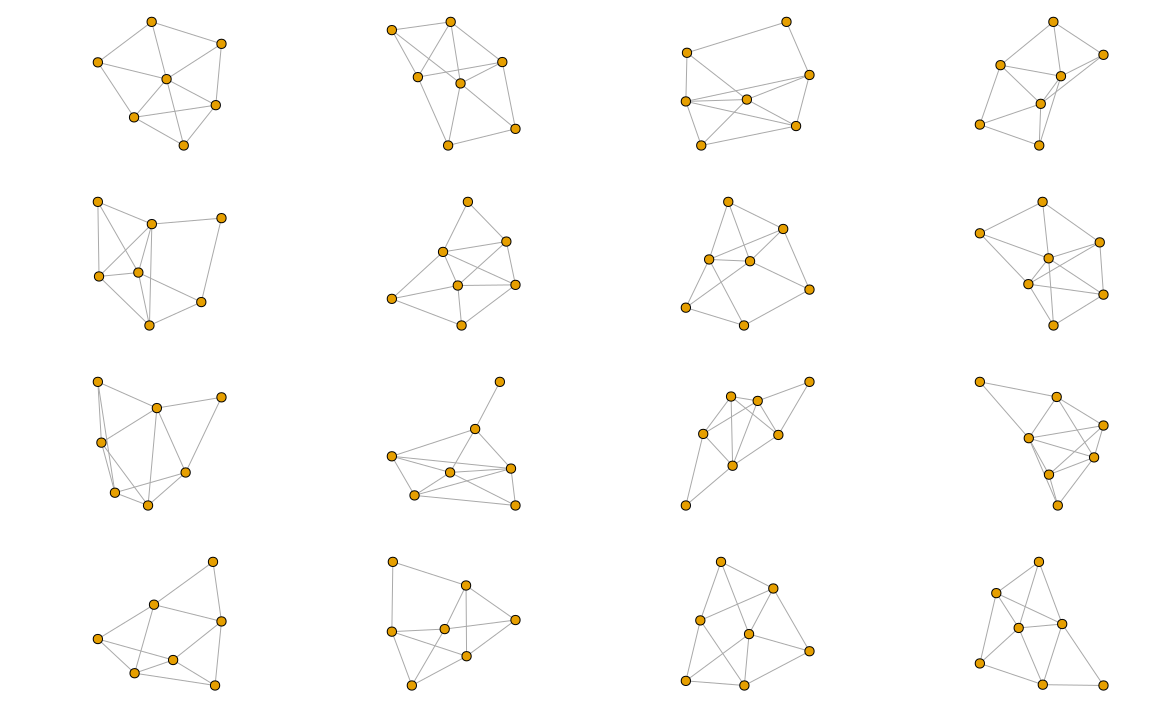
\includegraphics[width=0.95\linewidth]{atlas/atlas7-13.png}}
\end{figure}

\begin{figure}[h!]
	\subfloat
	{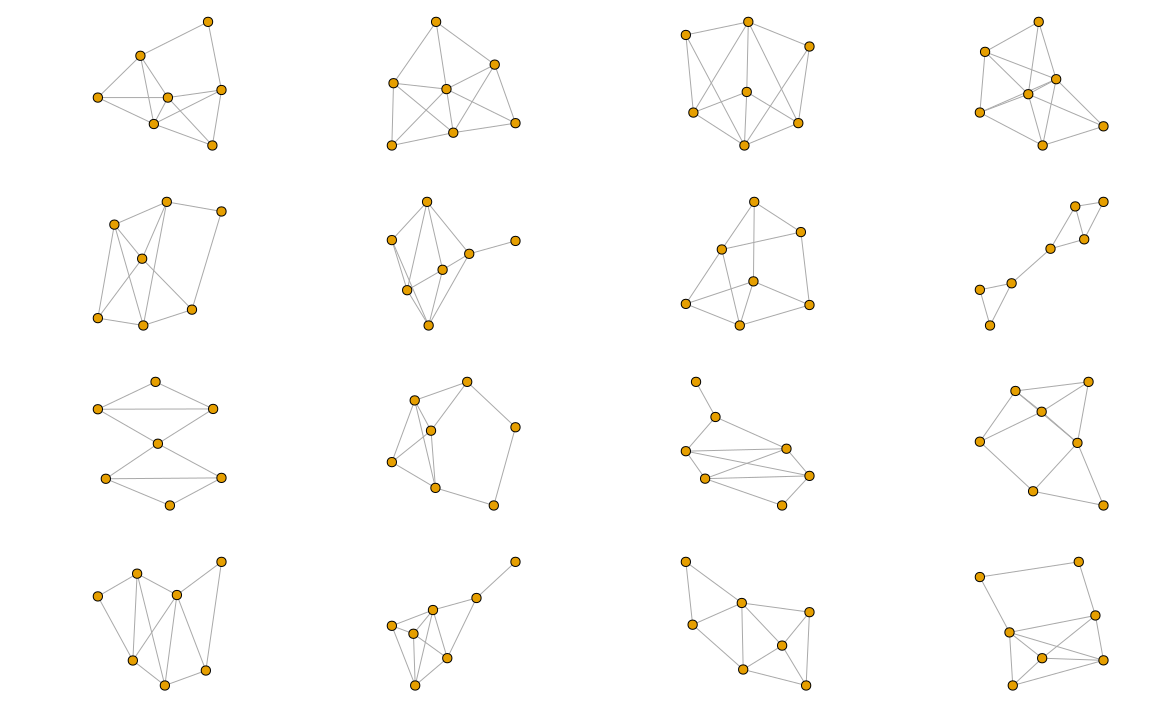
\includegraphics[width=0.95\linewidth]{atlas/atlas7-14.png}} \\
	\subfloat
    {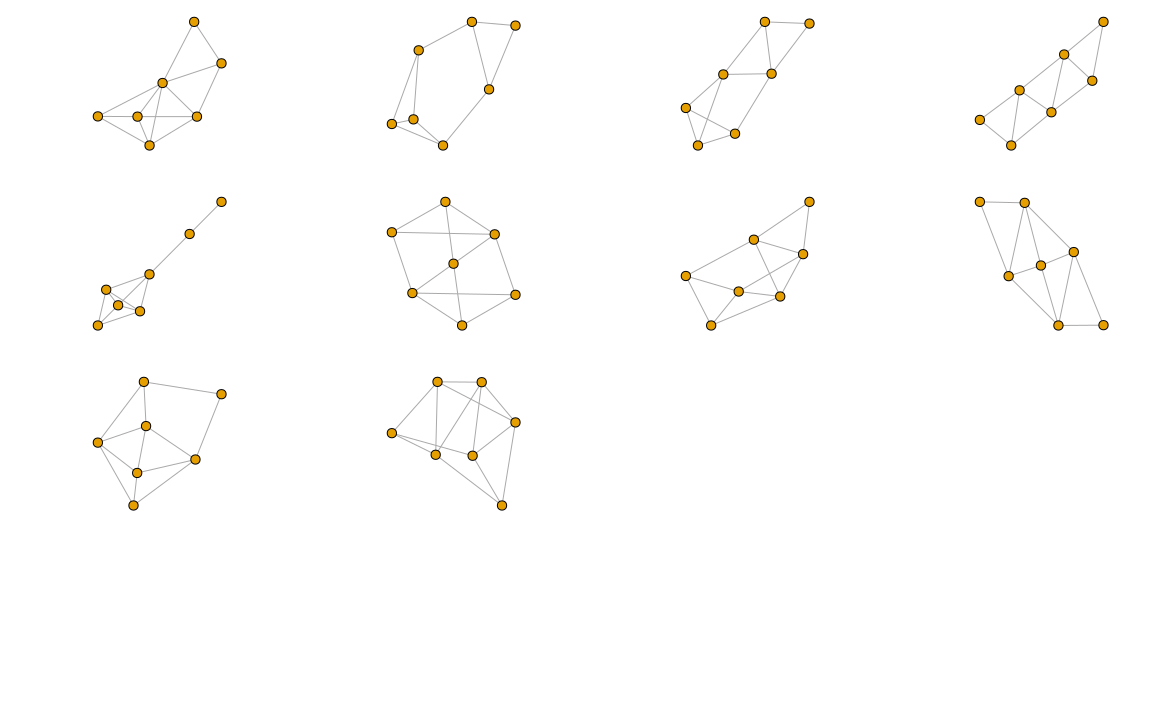
\includegraphics[width=0.95\linewidth]{atlas/atlas7-15.png}}
\end{figure}